
\begin{frame}{Accounting for individual characteristics}
\alert{\textbf{Route A}}: \newline
\begin{enumerate}
	\item Run on individual-level data:
	\beqns
		wage_{irt}^g=X_{iry}^g\gamma_t+\lambda_{rt}^g+\varepsilon_{irt}^g
	\eeqns
	\item In a second stage run:
	\beqns
		\hat{\lambda}_{rt}^{male}-\hat{\lambda}_{rt}^{female}=\tau_t+\beta_t\log(density)_{rt}+\varepsilon_{irt}^g
	\eeqns
\end{enumerate}
\end{frame}
\begin{frame}{Accounting for individual characteristics}
\alert{\textbf{Route B}}: \newline
If wages are determined at the individual level by the model:
\beqns
	w_{irt}^g=X_{irt}^g\gamma_t+\tau_tmale_i+\varepsilon_t
\eeqns
By aggregating at the CZ level this model becomes:
\beqns
w^{male}_{rt}-w^{female}_{rt}=\tau_t+ (\bar{X}_{rt}^{male}-\bar{X}_{rt}^{female})\gamma_t+u_t
\eeqns
Thus I run regressions of the form:
\beqns
w^{male}_{rt}-w^{female}_{rt}=\tau_t+ (\bar{X}_{rt}^{male}-\bar{X}_{rt}^{female})\gamma_t+\beta_t\log(density)_{rt}+u_t
\eeqns
\end{frame}
\begin{frame}{Route A}
\begin{figure}[!h]
\centering
\caption{Coefficient on population density $ \beta_t $ controlling for worker characteristics}
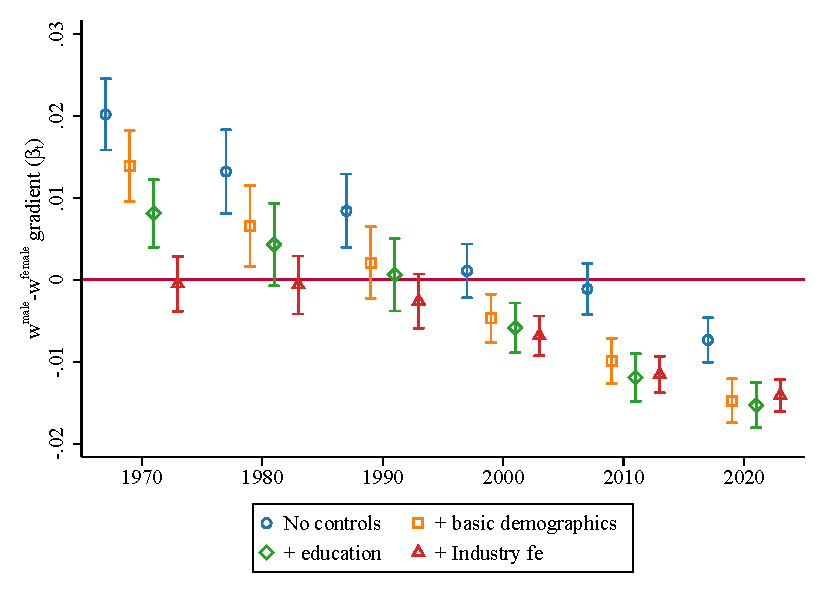
\includegraphics[width=.6\textwidth]{../2_analysis/output/figures/with_control_gradients_individual_l_czone_density_full_time}
\par \begin{minipage}[h]{\textwidth}{\tiny\textbf{Note:} figure restricts to CZ with more than 1 people per km$^2$. The regressions are done on data aggregated at the CZ level after residualizing individual-level characteristics. Bars show 95\% confidence intervals. Errors clustered at the CZ-level.}\end{minipage}
\end{figure}

\end{frame}
\begin{frame}{Route B}
\begin{figure}[!h]
\centering
\caption{Coefficient on population density $ \beta_t $ controlling for worker characteristics}
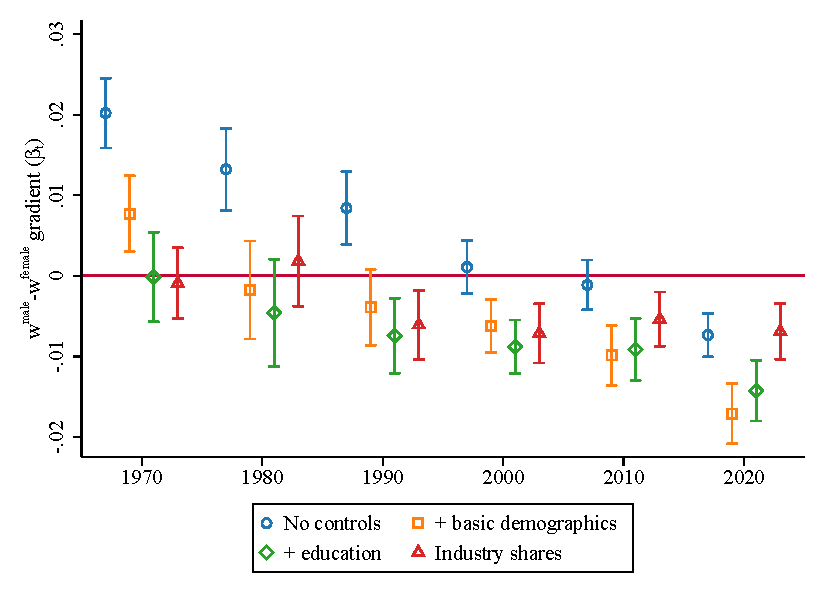
\includegraphics[width=.6\textwidth]{../2_analysis/output/figures/with_control_gradients_l_czone_density_full_time}
\par \begin{minipage}[h]{\textwidth}{\scriptsize\textbf{Note:} figure restricts to CZ with more than 1 people per km$^2$. The regressions are done on data aggregated at the CZ level. Bars show 95\% robust confidence intervals.}\end{minipage}
\end{figure}

\end{frame}